\documentclass{beamer}
\usetheme{Madrid}
\usecolortheme{seahorse}
\usepackage{amsmath, amssymb}

\title[Minimum Variance in Biased Estimation]{Minimum Variance in Biased Estimation: \\ Bounds and Asymptotically Optimal Estimators}
\author{\textit{Author} \\ Yonina C. Eldar \\ \vspace{+7pt}\textit{Presented by} \\ Aristeidis Daskalopoulos (10640) \\ Georgios Rousomanis (10703)}
\institute{IEEE Transactions on Signal Processing, July 2004}
\date{}

\begin{document}

% Customize footer: explicitly rewrite title and authors
\setbeamertemplate{footline}{
  \leavevmode%
  \hbox{%
    \begin{beamercolorbox}[wd=.3\paperwidth, ht=2.5ex, dp=1ex, center]{author in head/foot}%
      \usebeamerfont{author in head/foot}Daskalopoulos, Rousomanis
    \end{beamercolorbox}%
    \begin{beamercolorbox}[wd=.6\paperwidth, ht=2.5ex, dp=1ex, center]{title in head/foot}%
      \usebeamerfont{title in head/foot}Minimum Variance in Biased Estimation, Yonina C. Eldar\hspace*{2em}
    \end{beamercolorbox}%
    \begin{beamercolorbox}[wd=.1\paperwidth, ht=2.5ex, dp=1ex, center]{author in head/foot}%
      \usebeamerfont{author in head/foot}\insertpagenumber
    \end{beamercolorbox}%
  }%
  \vskip0pt%
}

\begin{frame}
  \titlepage
\end{frame}

\begin{frame}{Motivation and Background}
  \begin{itemize}
    \item A common approach to developing well-behaved estimators
    in overparameterized estimation problems is to use \textit{regularization} techniques.
    \item Regularization reduces variance but introduces bias.
    \item Cramér–Rao Lower Bound (CRLB) assumes unbiased estimators.
    \item Need for bounds applicable to biased estimators.
  \end{itemize}
\end{frame}

\begin{frame}{Key Goals of the Paper}
  \begin{itemize}
    \item Develop Uniform Cramér–Rao Lower Bound (UCRLB) for biased estimators.
    \item Use Frobenius and spectral norms of the bias gradient matrix.
    \item Construct estimators (Tikhonov, shrunken, PML) that achieve the bounds.
  \end{itemize}
\end{frame}

\begin{frame}{Classical and Biased CRLB}
  \begin{itemize}
    \item Unbiased CRLB: $\operatorname{Var}(\hat{\mathbf{x}}) \geq \mathbf{J}^{-1}$
    \item Biased CRLB:
    \begin{equation*}
        \begin{aligned}
            \mathbf{b}(\mathbf{x}_0) &= \mathbb{E}[\hat{\mathbf{x}}] - \mathbf{x}_0 \\
            \operatorname{Cov}(\hat{\mathbf{x}}) &\geq (\mathbf{I} + \mathbf{D}) \mathbf{J}^{-1} 
            (\mathbf{I} + \mathbf{D})^* \triangleq \mathbf{C}(\mathbf{D}) \\
            \mathbf{D} &= \frac{\partial \mathbf{b}(\mathbf{x}_0)}{\partial \mathbf{x}}
        \end{aligned}
    \end{equation*}
    \item Biased CRLB does not depend directly on the bias but only on the bias gradient matrix!
    \item $D$ is invariant to a constant bias term so that in effect, it characterizes the part of the bias 
    that cannot be removed
  \end{itemize}
\end{frame}

\begin{frame}{Bias Gradient Matrix}
  \begin{itemize}
  \item Given a desired bias gradient, the biased CRLB serves as a bound on the smallest attainable variance.
  \item How to choose $\mathbf{D}$?
  \pause
  \item Instead, use norms of $\mathbf{D}$ to constrain variance
  \begin{itemize}
    \item Frobenius norm (average bias)
    \item Spectral norm (worst-case bias)
  \end{itemize}
  \item Uniform CRLB (UCRLB): is a bound on the smallest attainable
  variance that can be achieved using any estimator with bias gradient whose norm is bounded by a constant.
  \end{itemize}
\end{frame}

\begin{frame}{Bias Gradient Matrix (cont.)}
  \begin{itemize}
    \item Generally, minimizing the bias results in an increase in variance and vice versa.
    \item Tradeoff between bias and variance
    \item Minimize $\operatorname{Tr}[\mathbf{C}(\mathbf{D})]$ subject to some constraint on $\mathbf{D}$.
    \item How to develop a meaningful constraint on $\mathbf{D}$?
    \pause
    \begin{itemize}
    \item Worst Case Bias Constraint:
        \[
        D_{WC} = 
        \max_{\mathbf{z} \in \mathbb{C}^m, \, ||\mathbf{z}|| = 1} \mathbf{z}^* \mathbf{S} \mathbf{D}^* \mathbf{D} 
        \mathbf{S} \mathbf{z}, \quad S \geq 0
        \]
        \item Average Bias Constraint:
        \[
        D_{AVG} = \operatorname{Tr}(\mathbf{D}^*\mathbf{D W}), \quad \mathbf{W} \geq 0
        \]
    \end{itemize}
    
  \end{itemize}
\end{frame}

\begin{frame}{UCRLB with Average Bias Constraint}
\begin{itemize}
\item Minimize total variance $C(\mathbf{D}) = \text{Tr}((\mathbf{I} + \mathbf{D})\mathbf{J}^{-1}(\mathbf{I} + \mathbf{D})^*)$
\item Subject to average bias constraint:
\[ D_{\text{AVG}} = \text{Tr}(\mathbf{D}^*\mathbf{D}\mathbf{W}) \leq \gamma \]
\item $\mathbf{W}$ is a non-negative Hermitian weighting matrix
\item $\mathbf{J}$ is the Fisher information matrix
\item $\mathbf{D}$ is the bias gradient matrix
\end{itemize}

\textbf{Key Insight:} The norm of the bias gradient matrix measures sensitivity of bias to parameter changes

\end{frame}

\begin{frame}{Theorem 1: UCRLB with Average Bias}
\begin{theorem}[Theorem 1]
For $\gamma < \text{Tr}(\mathbf{W})$, the total variance $C$ of any estimator with $\text{Tr}(\mathbf{D}^*\mathbf{D}\mathbf{W}) \leq \gamma$ satisfies:
\[ C \geq \alpha^2\text{Tr}((\mathbf{I} + \alpha\mathbf{W}\mathbf{J})^{-1}\mathbf{W}\mathbf{J}^{-1}\mathbf{W}(\mathbf{I} + \alpha\mathbf{J}\mathbf{W})^{-1}) \]
where $\alpha > 0$ is chosen such that:
\[ \text{Tr}((\mathbf{I} + \alpha\mathbf{W}\mathbf{J})^{-1}\mathbf{W}\mathbf{J}^{-1}(\mathbf{I} + \alpha\mathbf{J}\mathbf{W})^{-1}) = \gamma \]
\end{theorem}

\begin{itemize}
\item If $\mathbf{W} > 0$:
\[ C \geq \alpha^2\text{Tr}((\mathbf{W}^{-1} + \alpha\mathbf{J})^{-2}\mathbf{J}) \]

where  $\alpha > 0$ is chosen such that:
\[
\operatorname{Tr}((\mathbf{W}^{-1} + \alpha \mathbf{J})^{-2}\mathbf{W}^{-1}) = \gamma.
\]
\end{itemize}
\end{frame}

\begin{frame}{Comparison with UCRLB}
\begin{itemize}
    \item Until know we minimized the joint variance
    \item Scalar UCRLB minimizes variance for each component separately:
    \[
    \left[\mathbf{C}(\mathbf{D})\right]_{ii} = (\left[\mathbf{I}\right]_i^* + \mathbf{d}_i)\mathbf{J}^{-1}
    (\left[\mathbf{I}\right]_i + \mathbf{d}_i^*) \quad \text{s.t. } \mathbf{d}_i \mathbf{W} \mathbf{d}_i^* 
    \leq \gamma_i
    \]
    \item The total variance is:
    \begin{align*}
    \min_{\mathbf{D}} \left\{ \sum_{i=1}^{m} (\left[\mathbf{I}\right]_i^* + \mathbf{d}_i)\mathbf{J}^{-1}(\left[\mathbf{I}\right]_i +
    \mathbf{d}_i^*) \right\}
    &= \min_{\mathbf{D}} \left\{ \text{Tr}\left((\mathbf{I}+\mathbf{D})\mathbf{J}^{-1}(\mathbf{I} +
    \mathbf{D})^*\right) \right\} \\
    &= \min_{\mathbf{D}} C(\mathbf{D})
    \end{align*}

    Thus, we have the same optimization problem!
    
\end{itemize}
\end{frame}

\begin{frame}{Comparison with UCRLB (cont.)}
\begin{itemize}
    \item Scalar UCRLB minimizes $\mathbf{C}(\mathbf{D})$ s.t. 
    \[[\mathbf{D}\mathbf{W}\mathbf{D}^*]_{ii} \leq \gamma_i, \quad 1 \leq i \leq m.\]
    \item Vector UCRLB minimizes $\mathbf{C}(\mathbf{D})$ s.t. 
    \[\sum_{i=1}^m[\mathbf{D}\mathbf{W}\mathbf{D}^*]_{ii} \leq \sum_{i=1}^m\gamma_i = \gamma, 
    \quad 1 \leq i \leq m.\]
    \item Scalar constraints are tighter for the same optimization problem.
    \item Joint optimization over \( \mathbf{D} \) yields lower overall variance
    \item Cross-correlation allows bias in one component to reduce total variance by compensating for another.
\end{itemize}
\end{frame}

\begin{frame}{UCRLB with Worst-Case Bias Constraint}
\begin{itemize}
\item Minimize total variance $C(\mathbf{D}) = \text{Tr}((\mathbf{I}+\mathbf{D})\mathbf{J}^{-1}(\mathbf{I}+\mathbf{D})^*)$
\item Subject to worst-case bias constraint:
\[ D_{\text{WC}} = \max_{\mathbf{z}\in\mathbb{C}^m,\|\mathbf{z}\|=1} \mathbf{z}^*\mathbf{S}\mathbf{D}^*\mathbf{D}\mathbf{S}\mathbf{z} \leq \gamma \]

\item Two solution approaches:
\begin{enumerate}
\item \textbf{Jointly diagonalizable case}: Analytical solution via eigen-decomposition
\[ \mathbf{J}^{-1} = \mathbf{Q}\mathbf{\Lambda}\mathbf{Q}^*, \quad \mathbf{S} = \mathbf{Q}\mathbf{\Gamma}\mathbf{Q}^* \]
\item \textbf{Arbitrary $\mathbf{S}$ case}: Requires numerical SDP optimization
\end{enumerate}

\item Why consider jointly diagonalizable $\mathbf{S}$ and $\mathbf{J}$?
\pause
\begin{itemize}
\item[$\bullet$] Enables \textbf{closed-form solution} via eigendecomposition
\item[$\bullet$] Simplifies analysis by decoupling constraints along eigenvectors
\end{itemize}
\end{itemize}

\end{frame}

\begin{frame}{Worst-Case Constraint: Jointly Diagonalizable}
\begin{itemize}
\item Assume $\mathbf{S}$ and $\mathbf{J}$ share eigenvectors
\item Optimal bias gradient matrix:
\[ \hat{\mathbf{D}}_{\text{WC}} = (\mathbf{I} - \sqrt{\gamma}\mathbf{S}^{-1})\mathbf{P} - \mathbf{I} \]
where $\mathbf{P}$ is projection onto eigenvectors of $\mathbf{S}$ with $\beta_j^2 > \gamma$
\item Resulting total variance bound:
\[ \text{Tr}(\mathbf{C}_{\hat{\mathbf{x}}}) \geq \text{Tr}((\mathbf{I} - \sqrt{\gamma}\mathbf{S}^{-1})^2\mathbf{P}\mathbf{J}^{-1}) \]
\item Special case $\mathbf{S} = \mathbf{I}$:
\[ \text{Tr}(\mathbf{C}_{\hat{\mathbf{x}}}) \geq \text{Tr}((1 - \sqrt{\gamma})^2\mathbf{J}^{-1}) \]
\end{itemize}
\end{frame}

\begin{frame}{Worst-Case Constraint: Arbitrary $\mathbf{S}$}
\begin{itemize}
\item Assume that $\mathbf{S}$ is an arbitrary non-negative definite matrix
\item We formulate the minimization of $\mathbf{C}(\mathbf{D})$ as a semidefinite programming (SDP) problem:
\begin{align*}
\min_{t,\mathbf{D}} & t \\
\text{subject to} & \begin{bmatrix}
t & \mathbf{g}^* \\
\mathbf{g} & \mathbf{I}
\end{bmatrix} \succeq 0 \\
& \begin{bmatrix}
\gamma\mathbf{I} & \mathbf{S}\mathbf{D}^* \\
\mathbf{D}\mathbf{S} & \mathbf{I}
\end{bmatrix} \succeq 0
\end{align*}
where $\mathbf{g} = \text{vec}(\mathbf{J}^{-1/2}(\mathbf{I} + \mathbf{D})^*)$
\item Efficiently solvable using interior point methods
\end{itemize}
\end{frame}

\begin{frame}{Theorem 2: UCRLB with Worst-Case Bias}
\begin{theorem}[Theorem 2]
For $\gamma < \lambda_{\max}^2$, the total variance $C$ of any estimator with $\|\mathbf{D}\mathbf{S}\|^2 \leq \gamma$ satisfies $C \geq C_{\min}$, where $C_{\min}$ is the solution to the SDP problem.

For $\mathbf{S} = \sum \beta_i\mathbf{q}_i\mathbf{q}_i^*$ (same eigenvectors as $\mathbf{J}$):
\[ C_{\min} = \text{Tr}((\mathbf{I} - \sqrt{\gamma}\mathbf{S}^{-1})^2\mathbf{P}\mathbf{J}^{-1}) \]

For $\mathbf{S} = \mathbf{I}$:
\[ C_{\min} = \text{Tr}((1 - \sqrt{\gamma})^2\mathbf{J}^{-1}) \]
\end{theorem}

\textbf{Note:} From Theorems 1 and 2 the two UCRLB bounds coincide for the scalar case.
\end{frame}

%%%%%%%%%%%%%%%%%%%%%%%%%%%%%%%%%%%%%%%%%%%%%%%%%%%%%%%%%%%%%%%%%%%%%%%%%%%%%%%%%%%%%%%%%%%%%%%%%%%%%%%%

\begin{frame}{Optimal Estimators for the Linear Gaussian Model}
\begin{itemize}
    \item The described theorems, 1 and 2, characterize the smallest possible total variance of any estimator -- 
        \textit{with bias gradient matrix whose norm is bounded by a constant}.
    \item They do not guarantee that there exists estimators achieving these lower bounds.
    \item Now, we will show that for the case of a linear Gaussian model \textit{both lower bounds} are achievable using a linear estimator.
\end{itemize}
\pause
So, we consider the class of estimation problems represented by the linear model:
\[ \mathbf{y} = \mathbf{H} \mathbf{x_0} + \mathbf{n} \]

\scriptsize
\begin{itemize}
    \item \( \mathbf{x_0} \in \mathbb{C}^n \) is a deterministic vector of unknown parameters
    \item  \( \mathbf{H} \) is a known \( n \times m \) matrix with rank \( m \)
    \item \( \mathbf{n} \in \mathbb{C}^n \) is a zero-mean Gaussian random vector with positive definite covariance \( \mathbf{C_n} \).
\end{itemize}
\end{frame}


\begin{frame}{Optimal Estimators for the Linear Gaussian Model (cont.)}
\[ \text{Linear Model: } \ \mathbf{y} = \mathbf{H} \mathbf{x_0} + \mathbf{n} \]

\begin{itemize}
    \item For this model, the Fisher information matrix is given by:
        \[ \mathbf{J} = \mathbf{H}^*\mathbf{C_n}^{-1}\mathbf{H}. \]
    \item Let \( \hat{\mathbf{D}} \) denote the optimal gradient bias that minimizes \( \mathbf{C}(\mathbf{D}) \) subject to the Worst-Case \textit{or} Average Bias constrains. 
    \item Then, the total variance of any linear or nonlinear estimator \( \hat{\mathbf{x}} \) of \( \mathbf{x_0} \) is bounded by:
        \[ \text{Tr}(\mathbf{C_{\hat{x}}}) \geq \text{Tr}\left((\mathbf{I} + \hat{\mathbf{D}}) (\mathbf{H}^*\mathbf{C_n}^{-1}\mathbf{H})^{-1}(\mathbf{I} + \hat{\mathbf{D}})^*\right). \]
    \item We now derive a linear estimator \(\hat{\mathbf{x}} = \mathbf{G} \mathbf{y}\) of \(\mathbf{x}_0\) that achieves the above bound.
    \item Let: $\mathbf{G} = (\mathbf{I} + \hat{\mathbf{D}})(\mathbf{H}^* \mathbf{C}_n^{-1} \mathbf{H})^{-1} \mathbf{H}^* \mathbf{C}_n^{-1}.$
\end{itemize}
\end{frame}


\begin{frame}{Optimal Estimators for the Linear Gaussian Model (cont.)}
\[ \text{Linear Model: } \ \mathbf{y} = \mathbf{H} \mathbf{x_0} + \mathbf{n} \]
\[ \text{Linear Estimator: } \ \hat{\mathbf{x}} = \mathbf{G} \mathbf{y}, \quad \text{with } \  \mathbf{G} = (\mathbf{I} + \hat{\mathbf{D}})(\mathbf{H}^* \mathbf{C}_n^{-1} \mathbf{H})^{-1} \mathbf{H}^* \mathbf{C}_n^{-1}\]

\begin{itemize}
    \item The bias of this estimator is \(\mathbf{b} = (\mathbf{GH} - \mathbf{I}) \mathbf{x}_0\) so that the bias gradient matrix is:
        \[\mathbf{D} = \mathbf{GH} - \mathbf{I} = \hat{\mathbf{D}}\]
        which satisfies the Worst-Case \textit{or} Average Bias constrains.
    \item The total variance of \(\hat{\mathbf{x}} = \mathbf{G} \mathbf{y}\) is:
        \[\text{Tr}(\mathbf{C}_{\hat{\mathbf{x}}} ) = \text{Tr}(\mathbf{G} \mathbf{C}_n \mathbf{G}^*)
        = \text{Tr}\left((\mathbf{I} + \hat{\mathbf{D}})(\mathbf{H}^* \mathbf{C}_n^{-1} \mathbf{H})^{-1}(\mathbf{I} + \hat{\mathbf{D}})^*\right)\]
        so this estimator achieves the lower bound.  
    \item Note that the chosen estimator achieves the biased CRLB for estimators with bias gradient \(\mathbf{D}\). Thus, in the case of a linear Gaussian model, the biased CRLB is always achieved by a linear estimator.
\end{itemize}
\end{frame}


\begin{frame}{Optimal Estimator in the Linear Gaussian Model (AVG)}
\begin{itemize}
    \item Goal: Minimize total variance of estimators \(\hat{\mathbf{x}}\) under a constraint on the \textbf{Average} weighted bias gradient.
    \item Constraint: \(\text{Tr}(\mathbf{D}^{*}\mathbf{D}\mathbf{W}) \leq \gamma < \text{Tr}(\mathbf{W})\)
    \item Optimal estimator:
    \[
    \hat{\mathbf{x}} =
    \begin{cases}
    \left( \mathbf{H}^{*}\mathbf{C}_{n}^{-1}\mathbf{H} + \delta \mathbf{W}^{-1} \right)^{-1} \mathbf{H}^{*}\mathbf{C}_{n}^{-1} \mathbf{y}, & 0 \le \gamma < \text{Tr}(\mathbf{W}) \\
    0, & \gamma \geq \text{Tr}(\mathbf{W})
    \end{cases},
    \]
    with regularization parameter \(\delta > 0\) chosen such that:
    \[
    \text{Tr}\left((\mathbf{W}^{-1} + \frac{1}{\delta}\mathbf{H}^{*}\mathbf{C}_{n}^{-1}\mathbf{H})^{-2} \mathbf{W}^{-1} \right) = \gamma
    \]
    \item Conclusion: This is the \textbf{ridge estimator} (Tikhonov regularization), which:
    \begin{itemize}
        \item Minimizes total variance among all (linear and nonlinear) estimators \textit{with bounded average bias gradient}.
        \item Remains optimal (among linear estimators) for any noise distribution.
    \end{itemize}
\end{itemize}
\end{frame}


\begin{frame}{Optimal Estimator in the Linear Gaussian Model (WC)}
\begin{itemize}
    \item Goal: Minimize total variance under \textbf{Worst-Case} bias gradient constraint:
    \vspace{-10pt}
    \[
    \mathbf{z}^{*} \mathbf{S} \mathbf{D}^{*} \mathbf{D} \mathbf{S} \mathbf{z} \leq \gamma < \lambda_{\max}^{2}, \quad \forall \mathbf{z}, \; \|\mathbf{z}^*\mathbf{z}\| = 1
    \]
    where \( \mathbf{S} \succ 0 \) and commutes with \( \mathbf{H}^{*}\mathbf{C}_{w}^{-1}\mathbf{H} \).
    \item Optimal estimator:
    \[
    \hat{\mathbf{x}} = 
    \begin{cases} 
    (\mathbf{I} - \sqrt{\gamma}\mathbf{S}^{-1})\mathbf{P}\left(\mathbf{H}^*\mathbf{C_n}^{-1}\mathbf{H}\right)^{-1}\mathbf{H}^*\mathbf{C_n}^{-1}\mathbf{y}, & 0 \leq \gamma < \lambda_{\text{max}}^2 \\ 
    0, & \gamma \geq \lambda_{\text{max}}^2 
    \end{cases},
    \]
    \begin{itemize}
        \item \(\mathbf{P}\): projection onto eigenspace of \(\mathbf{S}\) with eigenvalues s.t. \(\beta_i^2 > \gamma\)
        \item \(\mathbf{G}\): defined as in earlier optimal estimator formula, with \(\hat{\mathbf{D}} = \hat{\mathbf{D}}_{\text{WC}}\)
    \end{itemize}
    \item Special case: If \(\mathbf{S} = \mathbf{I}\), this becomes the \textbf{shrunken estimator} (scaled version of least-squares estimator).
    \item Conclusion:
    \begin{itemize}
        \item The above estimator minimizes total variance among all (linear and nonlinear) estimators \textit{with bounded worst-case bias gradient}.
        \item Remains optimal (among linear estimators) for any noise distribution.
        \item For general \(\mathbf{S}\), this is a generalization of the shrunken estimator.
    \end{itemize}
\end{itemize}
\end{frame}


\begin{frame}{Application to System Identification}
\begin{itemize}

\item \textbf{Model}: Noisy measurements of filtered signal
\[ y[k] = \sum_{m=0}^{n-1} h[m]u[k-m] + \eta[k], \quad 0 \leq k \leq n-1 \]
\item Matrix form: $\mathbf{y} = \mathbf{H}\mathbf{x}_0 + \mathbf{n}$ where:
\begin{itemize}
\item $\mathbf{H}$ is lower triangular convolution matrix
\item $\mathbf{x}_0 = [h[0], \ldots, h[n-1]]^T$ (unknown impulse response)
\item $\mathbf{n} \sim \mathcal{N}(0,\sigma^2\mathbf{I})$ (white Gaussian noise)
\end{itemize}

\item \textbf{Note:} Since we have a linear Gaussian model, the UCRLB is achievable using a 
linear estimator. 

\item \textbf{Two Estimators}:
\begin{enumerate}
\item Vector Tikhonov (joint estimation):
\[ \hat{\mathbf{x}}_{\text{vec}} = \alpha(\alpha\mathbf{H}^*\mathbf{H} + \sigma^2\mathbf{I})^{-1}\mathbf{H}^*\mathbf{y},  \ 
\scriptstyle \text{where `$a$' chosen s.t. } \operatorname{Tr}((\mathbf{I} + \alpha/\sigma^2 \mathbf{H}^*\mathbf{H})^{-2}) = \gamma.
\]
\item Scalar Tikhonov (component-wise):
\[ \hat{x}_i = \alpha[(\alpha\mathbf{H}^*\mathbf{H} + \sigma^2\mathbf{I})^{-1}]_i^{-1}\mathbf{H}^*\mathbf{y}, \ 
\scriptstyle \text{where `$a$' chosen s.t. } [(\mathbf{I} + \alpha/\sigma^2 \mathbf{H}^*\mathbf{H})^{-2}]_{ii} = \frac{\gamma}{n}.
\]
\end{enumerate}
\end{itemize}
\end{frame}


\begin{frame}{Application to System Identification (cont.)}
\begin{columns}[T]
    \begin{column}{0.5\textwidth}
        \textbf{Observations}:
        \begin{itemize}
            \item Vector estimator achieves lower total variance for same bias gradient norm
            \item Performance gap increases with constraint tightness ($\gamma$)
            \item Empirical results match theoretical UCRLB predictions for both scalar and vector estimator
        \end{itemize}
        \vspace{0.3cm}
        \textbf{Key Insight:} Joint parameter estimation with vector constraint outperforms 
        component-wise scalar constraints
    \end{column}
    \begin{column}{0.5\textwidth}
        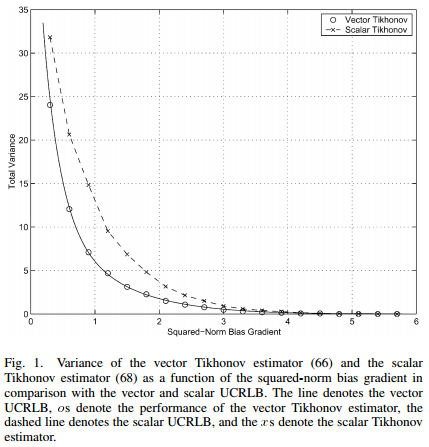
\includegraphics[width=\linewidth]{figures/fig1.png}
    \end{column}
\end{columns}
\end{frame}



%%%%%%%%%%%%%%%%%%%%%%%%%%%%%%%%%%%%%%%%%%%%%%%%%%%%%%%%%%%%%%%%%%%%%%%%%%%%%%%%%%%%%%%%%%%%%%%%%%%%%%%%%%%%

\begin{frame}{Asymptotic Optimality of the PML Estimator}
\begin{itemize}
    \item In general, the UCRLB may not be achievable.
    \item In the linear Gaussian model:
    \begin{itemize}
        \item With \underline{average} bias constraint, the \textbf{Tikhonov (ridge)} \textit{estimator achieves the UCRLB}:
        \[
        \hat{\mathbf{x}} = \arg\max\left\{\log p(\mathbf{y}; \mathbf{x}) - \frac{\beta}{2} \mathbf{x}^{*} \mathbf{W} \mathbf{x} \right\}
        \]
        \item Equivalent to minimizing: $(\mathbf{y} - \mathbf{H}\mathbf{x})^{*} \mathbf{C}_{n}^{-1} (\mathbf{y} - \mathbf{H}\mathbf{x}) + \beta \mathbf{x}^{*} \mathbf{W} \mathbf{x}$
        \item With \underline{worst-case} bias and \( \mathbf{S} = \mathbf{I} \) (or if $\mathbf{S}$ has same eigenvectors as $\mathbf{J}$), \textbf{shrunken estimator} also achieves the UCRLB (with: $\mathbf{W} = -\mathbf{H}^{*}\mathbf{H}$).
    \end{itemize}
    \item Conclusion: In linear Gaussian models, the PML estimator with suitable penalty achieves the UCRLB.
    \item Extension: The PML estimator asymptotically achieves the UCRLB in many \textit{general statistical models}, given an appropriate penalizing function.
\end{itemize}
\end{frame}


\begin{frame}{A. PML Estimator}
\begin{itemize}
    \item The PML estimator maximizes a penalized log-likelihood:
    \[
    \hat{\mathbf{x}}^{\text{PML}} = \arg\max \left\{ \log p(\mathbf{y}; \mathbf{x}) - \beta R(\mathbf{x}) \right\}
    \]
    where \( \beta > 0 \) for regularization, and \( R(\mathbf{x}) \) is a penalizing function.
    \item Interpretation: Equivalent to MAP estimation with prior pdf of $\mathbf{x}_0$ 
        \vspace{-5pt}
        \[ 
        p(\mathbf{x}) \propto e^{-\beta R(\mathbf{x})}. 
        \]
    \item For \(N\) \underline{iid} measurements \( \mathbf{y}_1, \ldots, \mathbf{y}_N \), the PML becomes:
    \[
    \hat{\mathbf{x}}^{\text{PML}} = \arg\max \left\{ \sum_{i=1}^{N} \log p(y_i; \mathbf{x}) - \beta_N R(\mathbf{x}) \right\}
    \]
    \item Many penalization forms exist, but... \\ general optimality is \textbf{not} guaranteed for these different choices!
    \item However, under certain regularity conditions:
    \begin{itemize}
        \item The PML estimator, from \( \mathbf{y}_1, \ldots, \mathbf{y}_N \) iid, is \textit{asymptotically Gaussian}.
        \item Explicit asymptotic mean and variance expressions can be derived.
        \item The PML asymptotically achieves the UCRLB.
    \end{itemize}
\end{itemize}
\end{frame}


\begin{frame}{B. Asymptotic Properties of the PML Estimator}
\begin{itemize}
    \item Goal: Estimate deterministic vector \( \mathbf{x}_0 \) from \( N \) iid measurements \( \mathbf{y}_1, \ldots, \mathbf{y}_N \) via the PML estimator, for: \\
    \begin{itemize}
        \item \( \beta_N \) s.t. \( \beta_N / N \to \beta_0 \) for some constant \( \beta_0 \) as \( N \to \infty \)
        \item \( R(\mathbf{x}) \) s.t. \( \partial^3 R(\mathbf{x})/\partial x_j \partial x_k \partial x_l \) is bounded for all \( j, k, l \)
    \end{itemize}
    \pause
    \item Assumptions on the pdf \( p(\mathbf{y}; \mathbf{x}) \):
    \begin{itemize}
        \item \textbf{A1:} First, second, and third(\( \partial^3 \log p(\mathbf{y}; \mathbf{x})/\partial x_j \partial x_k \partial x_l \)) derivatives of \( \log p(\mathbf{y}; \mathbf{x}) \) exist on open \( \mathcal{X} \ni \check{\mathbf{x}} \), where
        \[
        \check{\mathbf{x}} = \arg\max \left\{ E \left[ \log p(\mathbf{y}; \mathbf{x}) \right] - \beta_0 R(\mathbf{x}) \right\}
        \]
        \item \textbf{A2:} Third derivatives of \( \log p(\mathbf{y}; \mathbf{x}) \) are bounded by \( d(\mathbf{y}) \) with \( E_{\mathbf{x}}[d(\mathbf{y})] < \infty \), \( \forall \mathbf{x} \in \mathcal{X} \)
        \item \textbf{A3: } \(
        -E \left[ \frac{\partial^2 \log p(\mathbf{y}; \check{\mathbf{x}})}{\partial \mathbf{x}^2} \right] + \beta_0 \frac{\partial^2 R(\mathbf{x})}{\partial \mathbf{x}^2} > 0
        \)
    \end{itemize}
    \pause
    \item \textbf{Theorem 3:} Under A1--A3, the PML estimator is asymptotically normal:
    \[
    \sqrt{N}(\mathbf{\hat{x}}^{\text{PML}} - \check{\mathbf{x}}) \overset{a}{\sim}
    \mathcal{N}\left(0, (\mathbf{J}(\check{\mathbf{x}}) + \beta_0 \mathbf{M}(\check{\mathbf{x}}))^{-1} \mathbf{C}(\check{\mathbf{x}}) (\mathbf{J}(\check{\mathbf{x}}) + \beta_0 \mathbf{M}(\check{\mathbf{x}}))^{-1}\right)
    \]
    where $\beta_0 = \lim_{N \rightarrow \infty} \beta_N/N$.
\end{itemize}
\end{frame}


\begin{frame}{C. PML Estimator and the UCRLB}
\begin{itemize}
    \item From Theorem 3, the \textit{asymptotic} total variance of $ \mathbf{\hat{x}}^{\text{PML}} $ is
    \begin{equation*}
    \frac{1}{N} \text{Tr} \left( (\mathbf{J}(\check{\mathbf{x}}) + \beta_0 \mathbf{M}(\check{\mathbf{x}}))^{-1} \mathbf{C}(\check{\mathbf{x}}) (\mathbf{J}(\check{\mathbf{x}}) + \beta_0 \mathbf{M}(\check{\mathbf{x}})) \right), \quad \text{where: }
    \end{equation*}
    \[
    \check{\mathbf{x}} = \arg\max\{E \{\log p(\mathbf{y}; \mathbf{x})\} - \beta_0 R(\mathbf{x})\},
    \]
    \[
    \mathbf{C}(\check{\mathbf{x}}) = \text{cov}\left\{\frac{\partial \log p(\mathbf{y}; \check{\mathbf{x}})}{\partial \mathbf{x}}\right\}, \quad
    \mathbf{J}(\check{\mathbf{x}}) = -E\left\{\frac{\partial^2 \log p(\mathbf{y}; \check{\mathbf{x}})}{\partial \mathbf{x}^2}\right\},
    \]
    \[
    \text{and } \ \mathbf{M}(\check{\mathbf{x}}) = \frac{\partial^2 R(\check{\mathbf{x}})}{\partial \mathbf{x}^2}.
    \]

    \item From that we have that the \textit{asymptotic} bias gradient $\mathbf{D}_{\text{PML}}$ is
    \begin{equation*}
    \mathbf{D}_{\text{PML}} = \frac{\partial \check{\mathbf{x}}}{\partial \mathbf{x}_0} - \mathbf{I}.
    \end{equation*}

    \item After calculations we find the $\partial \check{\mathbf{x}}/\partial \mathbf{x}_0 = (\partial \check{\mathbf{x}}/\partial \mathbf{x}) \cdot (\partial \mathbf{x}/\partial \mathbf{x}_0)$ to be:
    \begin{equation*}
        \frac{\partial \check{\mathbf{x}}}{\partial \mathbf{x}_0} = (\mathbf{J}(\check{\mathbf{x}}) + \beta_0 \mathbf{M}(\check{\mathbf{x}}))^{-1} \frac{\partial}{\partial \mathbf{x}_0} E \left\{ \frac{\partial \log p(\mathbf{y}; \check{\mathbf{x}})}{\partial \mathbf{x}} \right\}.
    \end{equation*}
    
\end{itemize}
\end{frame}

\begin{frame}{C. PML Estimator and the UCRLB (\& Theorem 1)}
\begin{itemize}
    \item Let $\gamma = \mathbf{D}_{\text{PML}}^{*} \mathbf{D}_{\text{PML}}$. Then, from Theorem 1, any estimator with bias gradient $\mathbf{D}$ satisfying $\text{Tr}(\mathbf{D}^{*}\mathbf{D}) \leq \text{Tr}(\gamma)$ must satisfy:
    \begin{equation*}
    C \geq \frac{\alpha^2}{N} \text{Tr}\left((\mathbf{I} + \alpha \mathbf{J}_1)^{-2} \mathbf{J}_1\right),
    \end{equation*}
    where: 
    \begin{itemize}
        \item $\alpha > 0$ s.t. \(
            \text{Tr}\left((\mathbf{I} + \alpha \mathbf{J}_1)^{-2}\right) = \text{Tr}\left(\left(\frac{\partial \check{\mathbf{x}}}{\partial \mathbf{x}_0} - \mathbf{I}\right)^* \left(\frac{\partial \check{\mathbf{x}}}{\partial \mathbf{x}_0} - \mathbf{I}\right)\right),
            \)
        \item $\mathbf{J}_1 = E\left\{\left(\frac{\partial \log p(\mathbf{y}_1;\mathbf{x}_0)}{\partial \mathbf{x}}\right)^* \left(\frac{\partial \log p(\mathbf{y}_1;\mathbf{x}_0)}{\partial \mathbf{x}}\right)\right\}$. \(\scriptstyle (\textit{Fisher information from a single observation})\)
    \end{itemize}

    \item Thus, if $R(\mathbf{x})$ is chosen such that 
    \[
    \text{Tr}\left((\mathbf{J}(\check{\mathbf{x}}) + \beta_0 \mathbf{M}(\check{\mathbf{x}}))^{-1} \mathbf{C}(\check{\mathbf{x}}) (\mathbf{J}(\check{\mathbf{x}}) + \beta_0 \mathbf{M}(\check{\mathbf{x}}))^{-1}\right) =
    \]
    \[
    \alpha^2 \text{Tr}\left((\mathbf{I} + \alpha \mathbf{J}_1)^{-2} \mathbf{J}_1\right),
    \]
    then the PML estimator achieves the UCRLB under the \textit{average} bias constraint, and asymptotically no estimator (linear nor non-linear) with $\mathbf{D}$ st: $\text{Tr}(\mathbf{D}^{*} \mathbf{D}) \leq \text{Tr}(\gamma)$ has lower total variance.
\end{itemize}
\end{frame}


\begin{frame}{C. PML Estimator and the UCRLB (\& Theorem 2)}
\begin{itemize}
    \item From Theorem 2, the variance of any estimate of \(\mathbf{x}_0\) with bias gradient \(\mathbf{D}\) such that \(\|\mathbf{D}\|^2 \leq \|\mathbf{D}_{\text{PML}}\|^2\) satisfies:
    \[C \geq \frac{1}{N} \operatorname{Tr} \left( (1 - \|\mathbf{D}_{\text{PML}}\|)^2 \mathbf{J}_1^{-1} \right), \  \text{where: } \mathbf{D}_{\text{PML}} = \frac{\partial \check{\mathbf{x}}}{\partial \mathbf{x}_0} - \mathbf{I}.\]

    \item We choose $R(\mathbf{x})$ such that:
    \[\operatorname{Tr} \left( (\mathbf{J}(\check{\mathbf{x}}) + \beta_0 \mathbf{M}(\check{\mathbf{x}}))^{-1} \mathbf{C}(\check{\mathbf{x}}) (\mathbf{J}(\check{\mathbf{x}}) + \beta_0 \mathbf{M}(\check{\mathbf{x}}))^{-1} \right)\]
    \[= \operatorname{Tr} \left( \left( 1 - \left\| \frac{\partial \check{\mathbf{x}}}{\partial \mathbf{x}_0} - \mathbf{I} \right\| \right)^2 \mathbf{J}_1^{-1} \right), \ \scriptstyle \textit{where \(\partial \check{\mathbf{x}} / \partial \mathbf{x}_0\) known}.\]
     
    \item Based on the above, the corresponding PML estimator achieves the UCRLB under the \textit{worst-case} bias constraint.
    \item Asymptotically, no other linear or nonlinear estimator exists with:
    \begin{itemize}
        \item A bias gradient $\mathbf{D}$ such that $\|\mathbf{D}\| \leq \|\mathbf{D}_{\text{PML}}\|$, and
        \item A smaller total variance than that of the PML estimator.
    \end{itemize}
\end{itemize}
\end{frame}

\begin{frame}{C. PML Estimator and the UCRLB (for scalar $x_0$)}
\begin{block}{Observation}
\begin{center}
The conditions that are found for each one of the Theorems 1 and 2 are not very insightful when it comes to choosing $R(\mathbf{x})$, so we seek now to estimate a \textit{scalar} \( x_0 \) from \( N \) iid measurements.
\end{center}
\end{block}

\begin{itemize}
    \item In this analysis, the average and worst-case UCRLB coincide, and the variance $C$ of any estimate of $x_0$ with bias gradient $D$ such that:
    \begin{equation*}
        D^2 \leq D_{\text{PML}}^2 = \left(\partial \check{x} / \partial x_0 - 1\right)^2,
    \end{equation*}
    satisfies the bound:
    \begin{equation*}
        C \geq \left(1 - \left| \frac{\partial \check{x}}{\partial x_0} - 1 \right| \right)^2 \cdot \frac{1}{N J_1}, \ \text{where:}
    \end{equation*}
    $J_1 = E \left\{ \left( \frac{\partial \log p(y; x_0)}{\partial x} \right)^2 \right\}$, $\check{x} = \arg\max \left\{ E\left\{\log p(y; x)\right\} - \beta_0 R(x) \right\}$.
\end{itemize}

\end{frame}


\begin{frame}{C. PML Estimator and the UCRLB (for scalar $x_0$ -- cont.)}

\begin{itemize}
    \item Recall the sensitivity of the regularized estimator $\check{x}$:
    \begin{equation*}
        \frac{\partial \check{x}}{\partial x_0} = \frac{1}{J(\check{x}) + \beta_0 M(\check{x})} \cdot \frac{\partial}{\partial x_0} E \left\{ \frac{\partial \log p(y; \check{x})}{\partial x} \right\},
    \end{equation*}
    where:
    \[
    J(\check{x}) = -E \left\{ \partial^2 \log p(y; \check{x}) / \partial x^2 \right\}, \quad
    M(\check{x}) = \partial^2 R(\check{x}) / \partial x^2,
    \]
    \[
    C(\check{x}) = \text{var} \left\{ \partial \log p(y; \check{x}) / \partial x \right\}.
    \]

    \item From Theorem 3, the asymptotic variance of the PML estimator is:
    \begin{equation*}
        C_{\text{PML}} = \frac{C(\check{x})}{N(J(\check{x}) + \beta_0 M(\check{x}))^2}.
    \end{equation*}

    \item So, if we can choose $R(x)$ such that:
    \begin{equation*}
        \left(1 - \left| \frac{\partial \check{x}}{\partial x_0} - 1 \right| \right)^2 \cdot \frac{1}{J_1}
        = \frac{C(\check{x})}{(J(\check{x}) + \beta_0 M(\check{x}))^2},
    \end{equation*}
    then the PML estimator \textit{achieves} the UCRLB for scalar $x_0$.
    
\end{itemize}

\vspace{-25pt}

$$\scriptstyle \textit{Note: A general condition under which the above is satisfied can be found in Appendix B.}$$

\end{frame}

\begin{frame}{Example: Exponential Mean Estimation}

\begin{itemize}
    \item Consider estimating an unknown deterministic scalar parameter from $N$ iid measurements of an exponential random variable.
    
    \item The pdf is $p(y_i; x_0) = x_0 e^{-y_i x_0}, \quad 1 \leq i \leq N, $ and $1/x_0 > 0.$

     \item The PML estimate $\hat{x}^{\text{PML}}$ is obtained by maximizing:
    \begin{equation*}
        PL(x) = N \log x - x \sum_{i=1}^{N} y_i - \beta_N R(x),
    \end{equation*}
    for $\beta_N > 0$ with $\beta_N/N \to \beta_0$ as $N \to \infty$.

    \item The goal is to choose $R(x)$ such that $\hat{x}^{\text{PML}}$ asymptotically achieves the UCRLB.

    \item After calculations we have that:
    \begin{align*}
        \frac{\partial \log p(y; \check{x})}{\partial x} - E \left\{ \frac{\partial \log p(y; \check{x})}{\partial x} \right\} &= \frac{1}{x_0} - y, \\
        \frac{\partial \log p(y; x_0)}{\partial x_0} &= \frac{1}{x_0} - y.
    \end{align*}

\end{itemize}

\end{frame}


\begin{frame}{Example: Exponential Mean Estimation (cont.)}

\begin{itemize}
    \item From the mathematical analysis, if $\partial \check{x}/\partial x_0 \leq 1$, then the resulting PML estimator asymptotically achieves the UCRLB.

    \item However, for finite $N$, the choice of $R(x)$ still significantly impacts performance.

    \item We have, after computations:
    \[\frac{\partial \check{x}}{\partial x_0} = \frac{\frac{1}{x_0^2}}{\frac{1}{\check{x}^2} + \beta_0 M(\check{x})}\]

    \item If $\partial R(\check{x})/\partial x, \partial^2 R(\check{x})/\partial x^2 \geq 0$, then from the definition of $\check{x}$ we have:
    \[\frac{1}{\check{x}} = \frac{1}{x_0} + \beta_0 \frac{\partial R(\check{x})}{\partial x} \geq \frac{1}{x_0},\]
    and by differentiating that we indeed conclude to $\partial \check{x}/\partial x_0 \leq 1$ which means the PML estimator is optimal.

    \item For instance, by choosing $R(x) = x$ or $R(x) = \log x$ we have in both cases estimators that asymptotically achieve the UCRLB.

\end{itemize}
\end{frame}


\begin{frame}{Example: Compare the Performance of PML Estimators}

\begin{itemize}
    \item For $R(x) = x$ we have:
    \[
    \hat{x}^{\text{PML}} = \arg\max\left\{N \log x - x \left( \sum_{i=1}^{N} y_i + \beta_N \right) \right\} = \frac{N}{\sum_{i=1}^{N} y_i + \beta_N}.
    \]
    
    \item For $R(x) = \log x$ we have:
    \[
    \hat{x}^{\text{PML}} = \arg \max \left\{ (N - \beta_N) \log x - x \sum_{i=1}^{N} y_i \right\} = \frac{N - \beta_N}{\sum_{i=1}^{N} y_i}.
    \]

\end{itemize}
We will compare the performance of the PML estimators above with the UCRLB, for different values of $N$.

\end{frame}

\begin{frame}{Example: Empirical Evaluation of PML Estimators}

\begin{itemize}
    \item We compare two PML estimators with the UCRLB across different sample sizes $N$ by estimating:
    \begin{itemize}
        \item Estimator variance $\hat{\sigma}^2$.
        \item Squared bias gradient $\hat{D}^2$.
    \end{itemize}
    Rather than attempting to determine these quantities analytically, we propose to estimate them from the measurements.

    \item To estimate the variance of each of the estimators (for each $\gamma$), we generate $L = 5000$ PML estimators.  
    
    \item Variance is estimated as:
    \[
        \hat{\sigma}^2 = \frac{1}{L} \sum_{i=1}^{L} \left((\hat{x}^{\text{PML}})^{(i)} - \bar{x}_{\text{PML}} \right)^2, 
    \]
    where $\bar{x}_{\text{PML}}$ is the sample mean of $(\hat{x}^{\text{PML}})^{(i)}$ (which denotes and $i$-th estimator).
\end{itemize}

\end{frame}

\begin{frame}{Example: Empirical Evaluation of PML Estimators (cont.)}

\begin{itemize}
    \item We compare two PML estimators with the UCRLB across different sample sizes $N$ by estimating:
    \begin{itemize}
        \item Estimator variance $\hat{\sigma}^2$.
        \item Squared bias gradient $\hat{D}^2$.
    \end{itemize}
    Rather than attempting to determine these quantities analytically, we propose to estimate them from the measurements. 

    \item Squared bias gradient is estimated by:
    \[
        \hat{D} = \frac{1}{L} \sum_{i=1}^{L} \left( \left((\hat{x}^{\text{PML}})^{(i)} - \zeta^{(i)}\right) \left( \frac{N}{x} - \sum_{j=1}^{N} y_j^{(i)} \right) \right) - 1,
    \]
    \[
    \text{where: } \ \zeta^{(i)} = \frac{1}{L-1} \left( \sum_{j=1}^{L} \hat{x}^{(j)} - \hat{x}^{(i)} \right).
    \]

    \item Conclusion: This empirical framework enables a practical assessment of how well each PML estimator approaches the UCRLB, especially for finite \( N \).
\end{itemize}

\end{frame}

\begin{frame}{Example: Comparison of PML Estimators}

\begin{itemize}
    \item The next figures show the estimated variance vs. squared bias gradient for the two PML estimators, and the UCRLB, for \( N = 10, 20, 30 \).
    
    \item \textbf{Key observations:}
    \begin{itemize}
        \item Even for small \( N \), the UCRLB closely approximates the estimator variance, especially when the squared bias gradient is large.
        \item For small bias gradients, actual variance often exceeds the bound -- partially due to higher estimation variance in this regime.
        \item As \( N \) increases, both PML estimators converge to the UCRLB across all bias levels.
    \end{itemize}
    
    \item For small \( N \), the estimator with $R(x) = x$ shows consistently lower variance compared to the other one, indicating better finite-sample performance.
\end{itemize}

\end{frame}

\begin{frame}{Example: Plots (for $N = 10$ and $N = 20$)}
\begin{figure}
    \centering
    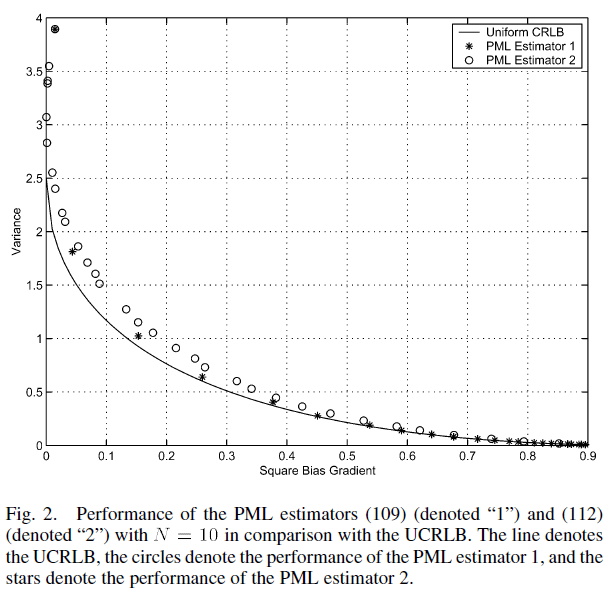
\includegraphics[width=0.45\textwidth]{figures/fig2.png}
    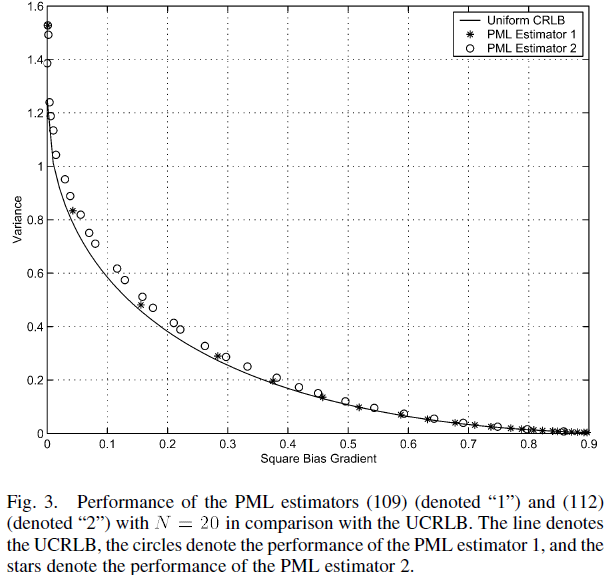
\includegraphics[width=0.45\textwidth]{figures/fig3.png}
\end{figure}
\end{frame}

\begin{frame}{Example: Plots (for $N = 20$ and $N = 30$)}
\begin{figure}
    \centering
    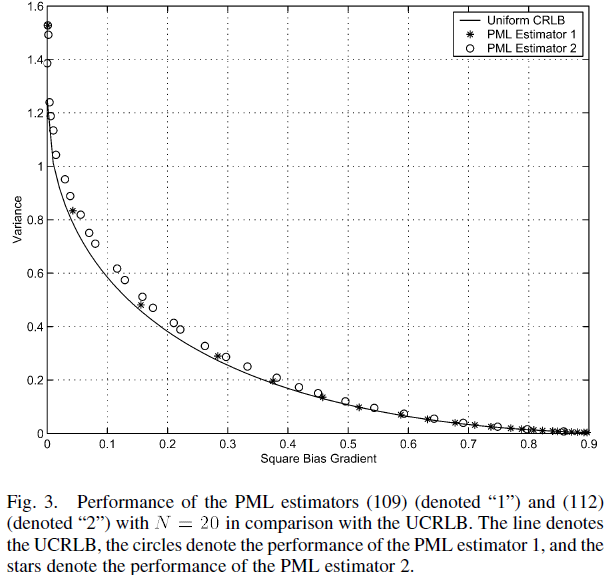
\includegraphics[width=0.45\textwidth]{figures/fig3.png}
    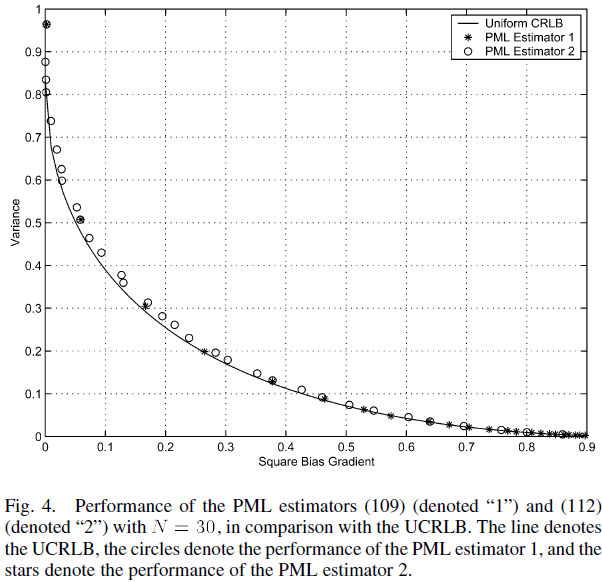
\includegraphics[width=0.45\textwidth]{figures/fig4.png}
\end{figure}
\end{frame}



\begin{frame}{Conclusions}
\begin{itemize}
    \item Developed lower bounds on the \textbf{total variance} of biased estimators by constraining the \textbf{bias gradient norm}.
    \item For the \textbf{linear Gaussian model}:
    \begin{itemize}
        \item \textbf{Tikhonov estimator} minimizes variance under average bias constraint.
        \item \textbf{Shrunken estimator} minimizes variance under worst-case bias constraint.
    \end{itemize}
    \item \textbf{PML estimator} with appropriate regularization:
    \begin{itemize}
        \item Asymptotically achieves the UCRLB.
        \item Varies in performance for finite sample sizes.
    \end{itemize}
    \item \textbf{Open Questions}:
    \begin{itemize}
        \item Can the PML achieve the UCRLB beyond the linear Gaussian model?
        \item How does the PML perform for \textit{finite} data?
        \item Can these results extend to cases where the Fisher Information Matrix is singular?
    \end{itemize}
\end{itemize}
\end{frame}




\begin{frame}{References}
  \scriptsize
  \begin{itemize}
    \item Hero et al., IEEE TSP, 1996
    \item Tikhonov, Sov. Math. Dokl., 1963
    \item Kay, Fundamentals of Statistical Signal Processing, 1993
    \item Eldar, IEEE TSP, 2004
    \item Fessler et al., IEEE Trans., multiple years
  \end{itemize}
\end{frame}

\begin{frame}{Q \& A}
  \centering
  Thank you for your attention! \\
  Questions and Discussion
\end{frame}

\end{document}
